\chapter{Activités confiées pendant le stage}
Pendant mon stage j'ai participé à beaucoup de fiches différentes, il serait long et ennuyeux de les détailler toutes sachant que je participai à entre 1 et 4 fiches par semaine. Je présenterai dans les grandes lignes les fonctionnalités majeure auxquelles j'ai participé.

\section{Découverte exploratoire de l'existant}
TODO

\section{Développements sur le code de production}
Parmi les activité qui m'ont été confiées, j'ai participé à la réalisation de fiches blanches (cf. \ref{agile:fiches} \pageref{agile:fiches}). Le code produit est appelé ``code de production'' car il couvre les besoins fonctionnels exprimés par le client XP. La première étape dans le travail sur une fiche est de préciser le périmètre fonctionnel avec le client XP. Ceci permet aux développeurs de connaitre son besoin précis. Ensuite, dans la mesure du possible, on crée les tests unitaires qui permettront de savoir si la fonctionalité est opérationnelle. Les membres du binôme peuvent prendre le clavier au moment où ils le souhaitent et proposer leurs idées. Chaque direction prise et ainsi refléchie et validée par chaque memebre du binôme.

\subsection{Observations}

\subparagraph*{}
Au début de mon stage, la première fonctionalité sur laquelle j'ai travaillé fut des observations. Dans le produit, le observations sont des stéréotypes attachés à des opérations du modèle de test. Les observation sont déclenchées par des triggers\footnote{Evènement déclencheur} selon une précondition décrite dans le langage OCL(cf. lexique \ref{lexique:OCL} p.\pageref{lexique:OCL}). Dans les modeleurs, à l'export, ce stéréotype est reconnu et intégré au modèle propre à Test Designer. Les observations font office de ``points de contrôle '' permettant de vérifier que le système sous test réagit correctement.

\subparagraph*{}
Les observations sont introduites dans les deux modeleurs principaux de façon différente. Dans RSM, les stéréotypes et la gestion des triggers spécifiques à SMARTESTING proviennent d'un profil personnalisé. L'utilisation des profils dans le modeleur Together ont été l'occasion d'une autre fiche à laquelle j'ai contribué. Cependant mon binôme et moi-même nous somme rendu compte, après avoir passé 4 points de vélocité sur cette fiche cotée à 2, que c'était plus compliqué que nous l'imaginions. Nous avons alors suspendu la fiche en attente de conseils d'OBEO\footnote{OBEO est une société de conseil experte dans le domaine de la modélisation EMF/GMF sous Eclipse}. Finalement la après leur réponse, nous avons dù Rollback(cf. lexique \ref{lexique:rollback} p.\pageref{lexique:rollback}) notre travail. La solution adaptée finalement fut d'utiliser le code péexistant. C'est à dire utiliser des propriétés ``Custom''(cf. figure \ref{figure:obsTriggerTG} p.\pageref{figure:obsTriggerTG}) pour gérer les triggers dans Together. Ces triggers servent à déterminer les opérations que l'on souhaite observer. Une fois définies dans le modèle UML et après export, les observations sont visibles dans Test Designer (cf. figure\ref{figure:obsTD} p.\pageref{figure:obsTD}).

\begin{figure}[!h]
\centering
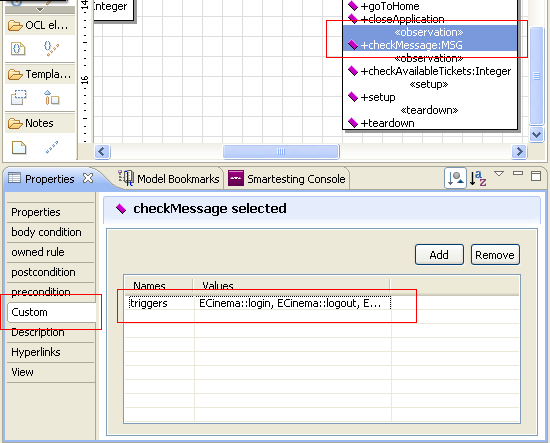
\includegraphics[scale=0.5]{Illustrations/Observation_Trigger_Together.png}
\caption{Intégration des observations dans Together}
\label{figure:obsTriggerTG}
\end{figure}

\begin{figure}[!h]
\centering
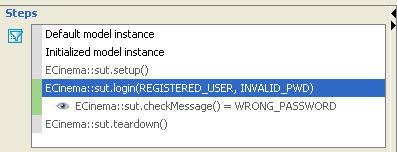
\includegraphics[scale=0.5]{Illustrations/Observation.png}
\caption{Intégration des observations dans Test Designer}
\label{figure:obsTD}
\end{figure}









fiche à laquelle j'ai participé traitait d'un bug d'IHM\footnote{Interface homme-machine}.TODO : Correction bug affichage no changes, travail sur Setup/teardown, 
\subsection{Documentation}

\subsection{Validation}
La validation des fiches est obligatoire pour considérer que la fonctionnalité lui correspondant est terminée. Elle consiste au test de la fonctionnalité sur l'application après commit. La validation se fait généralement en binôme et il faut chercher toutes les combinaisons en rapport avec la nouvelle fonctionnalité qui sont susceptible d'échouer, de vérifier si toutes les objectifs de la fiche sont remplis. Après avoir testé un maximum de cas de figures il faut faire appel au Client XP qui va s'assurer que l'engagement a été rempli. Une fois cela fait, la fiche est terminée et son nombre de points de vélocité peut être ajouté à ce qui a déjà été fait
\subsection{Amélioration du code existant (refactoring)}
TODO : utilité ,exemple, 
\subsection{Administration système}
Sur une courte période j'ai effectué des t\^aches d'administration système. En particulier au moment de l'intégration des Google Apps dans le fonctionnement de Smartesting. La necessité de partager des calendriers et de pouvoir y accéder via des plateformes mobiles a amené Smartesting à envisager d'utiliser Google Apps. Ainsi, en binôme avec Olivier, nous avons appréhendé le panneau d'administration ainsi que les différents services utilisables. Chaque calendrier donne la possibilité d'être exporté, ainsi nous avons pu réaliser une routine de backup\footnote{sauvegarde automatique}.
\subsection{Meeting corporate}
TODO : definition, utilité, ma participation ...
\subsection{Visite de BNP Paribas}
Mes impressions, les decisions, Smart et BNP ...

\subsection{Amélioration du process, évolution du fonctionnement de l'équipe}
J'ai été ammené à l'occasion de retrospectives ou de réunions à réfléchir sur le processus de développement au sein de l'équipe. L'équipe de R\&D est très concernée par l'amélioration du processus et toute pratique peut être remise en cause si elle ne convient pas a l'équipe. Chaque décision quelle qu'elle soit doit être approuvée par toute l'équipe avant d'être prise. Je parlerai plus en détail à travers d'exemple du type de décisions qui sont prises sur ce sujet.

Tableau des évolution des pratiques XP
\begin{table}[!ht]
	\caption{\label{tableau:evolPratXP}Evolution des pratiques XP au cours du stage}
	\begin{tabular}{|l|c|c|}
		\hline
		Pratique & Début du stage & Fin du stage\\
		\hline
		Pair programming & \tick & \tick \\
		Itération & 2 semaines & 1 semaine \\
		Intégration continue & \tick & \tick \\
		Niko Niko & \tick & \badtick \\
		Lecture & \tick & \badtick \\
		Point perso & hebdomadaire & nouvelles experimentations\\
		Pomodoro & \badtick & \tick \\
		Test driven development & \tick & \tick \\
		``Done done'' & théorique & adopté et normalisé\\
		``No Bugs'' & imprécis & engagement \\
		Slack Time & \badtick & adopté et normalisé\\
		Rétrospective & 1 à 2h le lundi matin & Timeboxée et juste après la livraison\\
		Point technique & assez réguliers & moins nombreux\\
		Veilleur & \tick & Robin cumule son rôle\\
		Batman/Robin & \badtick & \tick \\
		\hline
	\end{tabular}
\end{table}


TODO : Pomodoro, Decisions lors de retrospectives, Iteration 1 semaine, Slack, reduction de vélocité, Done-done, rédaction(et simplification) des standards, Objectifs R\& D, ...